
\subsection{Implement\'aci\'o}

\subsubsection{Architekt\'ura}
Az alkalmaz\'as k\'etr\'eteg\H u modell-n\'ezet architekt\'ura szerint k\'esz\"ult.
Ezek m\H uk\"od\'es\'et a \code{VisaulizationApplication} oszt\'aly k\"oti \"ossze \'es ir\'any\'itja.

\subsubsection{Alkalmaz\'as}
\begin{figure}[h]
	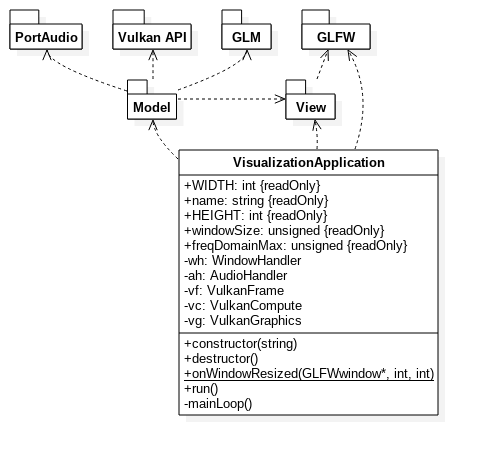
\includegraphics[width=\textwidth]{VisualizationApplication__VisualizationApp_0}
	\centering
	\caption{Az alkalmaz\'as oszt\'alydiagramja \'es a csomagkapcsolatok}
\end{figure}

Az alkalmaz\'as nev\'et a konstruktorban lehet be\'all\'itani, majd a \code{run} met\'odussal elind\'itani. \'Igy a \code{src/main.cpp} f\'ajlban tal\'alhat\'o \code{main} f\"uggv\'enynek csak az alkalmaz\'as futtat\'asa \'es a program sor\'an eldobott kiv\'etelek legv\'egs\H o elkap\'asa lesz a feladata.
Maga az alkalmaz\'as a k\"ovetkez\H o v\'altoz\'okon kereszt\"ul param\'eterezhet\H o:
\begin{itemize}
	\item \code{WIDTH} \'es \code{HEIGHT}: a megjelen\'it\H o ablak kezdeti m\'erete.
	\item \code{windowSize}: mekkora legyen a minta, amit elemz\"unk; a specifik\'aci\'oban $N$
\end{itemize}

\subsubsection{N\'ezet}
\begin{figure}[h]
	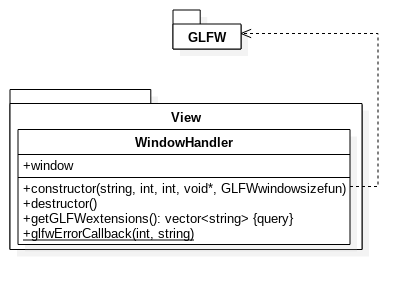
\includegraphics[width=\textwidth]{View__ViewClassDiagram_7}
	\centering
	\caption{A n\'ezet r\'eteg}
\end{figure}
Az alkalmaz\'as fel\"ulete egy darab megjelen\'it\H o ablakb\'ol \'all, ez a prezent\'aci\'os fel\"ulet.
Ezt a \code{WindowHandler} oszt\'aly biztos\'itja, a GLFW k\"onyvt\'ar seg\'its\'eg\'evel. \newline
A konstruktor\'aban inicializ\'alja a GLFW-t, l\'etrehozza \'es be\'all\'itja az ablakot, be\'all\'itja a hibakezel\H o f\"uggv\'eny\'et. \newline
A \code{getGLFWextensions} f\"uggv\'ennyel inform\'aci\'ot szerezhet\"unk a k\"onyvt\'art\'ol, hogy milyen kieg\'esz\'it\H o funkcionalit\'asokra lesz sz\"uks\'eg\"unk a z\"okken\H omentes m\H uk\"od\'eshez. Ezt felhaszn\'aljuk amikor egy kompatibilis fizikai eszk\"ozt keres\"unk.

\subsubsection{Modell}
\begin{figure}[h]
	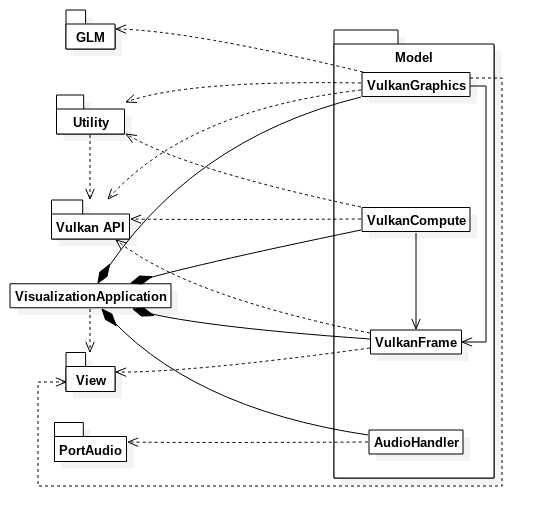
\includegraphics[width=\textwidth]{Model__ModelClassDiagram_1}
	\centering
	\caption{A modell r\'eteg kapcsolati \'abr\'aja}
\end{figure}
A modell r\'eteg tov\'abbi r\'eszekre bonthat\'o.

\paragraph{Hangkezel\'es}\label{audiohandling}
\begin{figure}[h]
	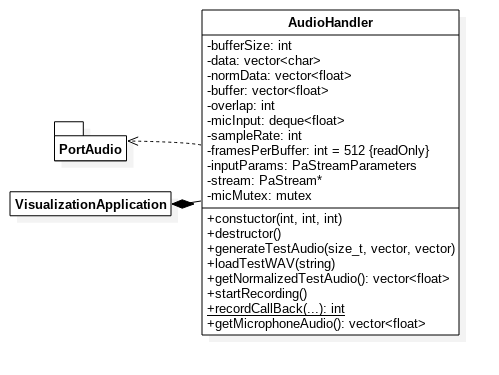
\includegraphics[width=\textwidth]{Model__AudioHandler_5}
	\centering
	\caption{Az \code{AudioHander} oszt\'alydiagramja}
\end{figure}
A hang kezel\'es\'et az \code{AudioHandler} oszt\'aly biztos\'itja.
A konstruktor\'aban lefoglal a t\'arol\'oknak helyet \'es inicializ\'alja a \code{PortAudio} k\"onyvt\'art.
H\'arom param\'eterrel tudjuk a m\H uk\"od\'es\'et finomhangolni:
\begin{itemize}
	\item A buffer m\'erete
	\item A mintav\'etelez\'esi r\'ata
	\item H\'any csatorn\'an t\"ort\'enik a mintav\'etelez\'es
\end{itemize}
Az ut\'obbi kett\"onek csak mikrofonbemenet haszn\'alata eset\'en van jelent\H os\'ege.
Az \code{overlap} adattag azt szab\'alyozza, hogy a v\'etlezett mint\'ak mekkora fed\'esben legyenek. $\code{overlap}\in[0..\code{bufferSize})$
%TODO: a r\'at\'at belevenni a f\'ajlbeolvas\'asba
\newline
Ezek ut\'an h\'aromf\'elek\'epp tud hangadatot szolg\'altatni:
\begin{enumerate}
	\item Harmonikus rezg\'esek line\'aris kombin\'aci\'ojak\'ent el\"o\'all\'it egy mesters\'eges \"osszetett hangot
		\begin{enumerate}
			\item A \code{generateTestAudio} f\"uggv\'enynek megadjuk, hogy mekkora intervallumon milyen frekvenci\'aj\'u \'es amplit\'ud\'oj\'u harmonikus rezg\'eseket \'all\'itson el\H o
			\item Majd a \code{getNormalizedTestAudio} f\"uggv\'ennyel tudjuk az el\H o\'all\'itott hang egy prefix\'et elk\'erni. A f\"uggv\'eny t\"orli ezt a prefixet.
		\end{enumerate}
	\item M\'ar l\'etez\H o \code{wav} f\'ajlt bet\"olt hangbemenetk\'ent
		\begin{enumerate}
			\item A \code{loadTestWAV} f\"uggv\'ennyel beolvassa a f\'ajlt.
			\item A \code{getNormalizedTestAudio} f\"uggv\'ennyel a beolvasott f\'ajlt egy prefix\'et elk\'erni. A f\"uggv\'eny t\"orli ezt a prefixet.
		\end{enumerate}
	\item Mikrofon \'altal \'eszlelt hangot haszn\'aljon.
		\begin{enumerate}
			\item A \code{startRecording} met\'odussal elind\'itja a PortAudio streamet.
			\item Ezut\'an a \code{getMicrophoneAudio} f\"uggv\'ennyel tudunk az \'eszlelt adatb\'ol olvasni.
		\end{enumerate}
\end{enumerate} 


\paragraph{Hangfeldolgoz\'as}
\begin{figure}[h]
	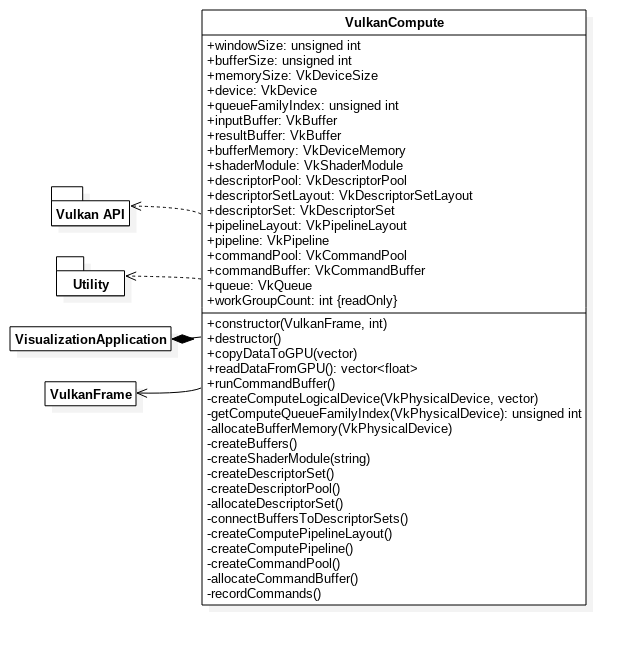
\includegraphics[width=\textwidth]{Model__VulkanCompute_3}
	\centering
	\caption{A \code{VulkanCompute} oszt\'alydiagramja}
\end{figure}
A hangfeldolgoz\'as a specifik\'aci\'oban eml\'itett m\'odon diszkr\'et Fourier-transzform\'aci\'oval t\"ort\'enik, ami a \code{VulkanCompute} oszt\'aly seg\'its\'eg\'evel vide\'ok\'arty\'an t\"ort\'enik.
A konstruktor\'aban l\'etrehozza a m\H uk\"od\'es\'ehez sz\"uks\'eges eszk\"oz\"oket. 
\begin{itemize}
	\item A logikai eszk\"ozt, amin kereszt\"ul a program a fizikai eszk\"ozzel kommunik\'alni tud.
	\item A logikai eszk\"ozh\"oz tartoz\'o sort, ahova az utas\'it\'asokat lehet k\"uldeni.
	\item Mem\'ori\'at allok\'al az eszk\"ozon.
	\item Buffereket hoz l\'etre a mem\'oria el\'er\'es\'ere.
	\item L\'etrehozza az er\H oforr\'as le\'ir\'okat.
	\item Bet\"olti a sz\'am\'it\'ast defini\'al\'o shadert.
	\item Sz\'am\'it\'asi szerel\H oszalagot hoz l\'etre.
	\item Command pool-t kre\'al \'es command buffer-t foglal bel\H ole.
	\item Felveszi a majd v\'egrehajtand\'o parancsokat a command buffer-be.
\end{itemize}

Ezek ut\'an haszn\'alatra k\'esz, amely a k\"ovetkez\H o sorrendben t\"ort\'enik:
\begin{enumerate}
	\item Adatok felt\"olt\'ese a mem\'ori\'aba a \code{copyDataToGPU} f\"uggv\'eny seg\'its\'eg\'evel.
	\item A sz\'am\'it\'as futtat\'asa a \code{runCommandBuffer} met\'odus megh\'iv\'asa \'altal.
	\item A sz\'amolt eredm\'eny kiolvas\'as\'a a \code{readDataFromGPU} f\"uggv\'ennyel.
\end{enumerate}

\paragraph{Rajzol\'as}
\begin{figure}[h]
	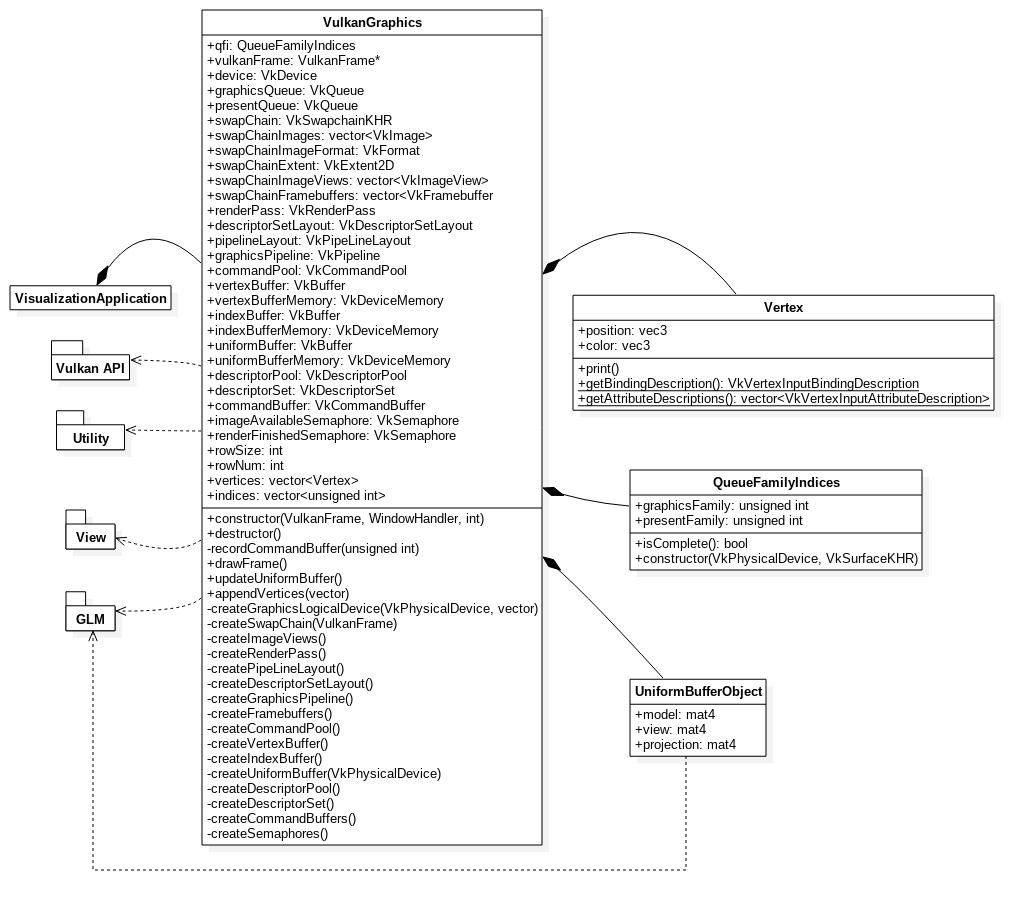
\includegraphics[width=\textwidth]{Model__VulkanGraphics_4}
	\centering
	\caption{A \code{VulkanGraphics} oszt\'alydiagramja}
\end{figure}
A kisz\'amolt amplit\'ud\'o \'ert\'ekeket a \code{VulkanGraphics} oszt\'aly seg\'its\'egevel tudjuk az ablakon megjelen\H o rajzz\'a alak\'itani. 
Inicializ\'al\'askor a sz\'am\'it\'asi egys\'eghez hasonl\'oan hoz l\'etre a m\H uk\"od\'es\'ehez sz\"uks\'eges eszk\"oz\"oket, csak mivel a megjelen\'it\'es \"osszetettebb feladat, ezek kieg\'esz\"ulnek, illetve m\'odusulnak.
\begin{itemize}
	\item L\'etrehoz egy rajzol\'as\'ert felel\H os logikai eszk\"ozt, amin kereszt\"ul a fizikai eszk\"ozzel lehet kommunik\'alni.
	\item Be\'all\'itja a rajzol\'o \'es a prezent\'al\'o sorokat.
	\item L\'etrehoz egy \code{swapchain}-t. Ez felel\H os a bufferek kezel\'es\'e\'ert. A jelenlegi implement\'aci\'o, amennyiben a hardver is t\'amogatja \code{double buffering}-et haszn\'al. Rajzol\'askor a \code{swapchain}-t\H ol kell k\'epet (pontosabban a k\'ep indexet) k\'erni, amire majd a rajz ker\"ul.
	\item L\'etrehozza a t\'enyleges k\'epeket, amikre rajzolni lehet.
	\item Be\'all\'it egy renderel\H o menetet.
	\item Defini\'alja az er\H oforr\'as le\'ir\'o s\'em\'at.
	\item Defini\'alja a szerel\H oszalag s\'em\'aj\'at.
	\item L\'etrehozza a grafikus szerel\H oszalagot.
	\item L\'etrehozza a \code{frame buffer}-eket, ami \"osszek\"oti a k\'epekkel a renderel\'est.
	\item L\'etrehozza az utas\'it\'as pool-t.
	\item Mem\'ori\'at allok\'al az eszk\"oz\"on a vertexeknek, indexeknek \'es a transzform\'aci\'os m\'atrixoknak, majd \"osszekapcsolja \H oket a megfelel\H o bufferekkel.
	\item Inicializ\'alja az er\H oforr\'asle\'ir\'o pool-t, majd allok\'alja bel\H ole a t\'enyleges er\H oforr\'as le\'ir\'okat.
	\item Lefoglal az utas\'it\'as pool-b\'ol utas\'it\'as buffert.
	\item L\'etrehozza a rajzol\'as folyamat\'an a helyes fut\'asi sorrend biztos\'it\'as\'ara haszn\'alt szemaforokat. 
\end{itemize}
Miut\'an sikeresen l\'etrej\"ott a \code{VulkanGraphics} objektum, a k\"ovetkez\H o m\'odon t\"ort\'enhet a haszn\'alata.
\begin{enumerate}
	\item Az \code{appendVertices} met\'odussal felt\"olti a vertexeket a \code{vertices} vektorba, illetve kisz\'amolja a rajzoland\'o h\'aromsz\"ogek cs\'ucspontvertexeinek indexeit \'es azokat felt\"olti az \code{indices} vektorba.
	\item Az \code{updateUniformBuffer} f\"uggv\'eny friss\'iti a transzform\'aci\'os m\'atrixokat.
	\item A \code{drawFrame} elj\'ar\'as pedig kirajzolja az aktu\'alis k\'epkock\'at.
		\begin{enumerate}
			\item Elk\'eri a k\'ep index\'et a swapchain-t\H ol. (aszinkron)
			\item Felt\"olti a \code{vertices} \'es az \code{indices} t\"omb tartalm\'at a a vide\'ok\'artya mem\'ori\'aj\'aba.
			\item Felveszi a utas\'it\'asbuffer-be a v\'egrehajtand\'o utas\'it\'asokat.
			\item Elk\"uldi a grafikus sornak az utas\'it\'ast v\'egrehajt\'asra. (aszinkron)
			\item Felk\'esz\"ul az elk\'esz\"ult k\'ep prezent\'al\'as\'ara, \'es amint a \code{renderFinishedSemaphore} jelez, hogy elk\'esz\"ult a renderel\'es, kirakja megjelen\'it\H o fel\"uletre az elk\'esz\"ult k\'epet.
		\end{enumerate}
\end{enumerate}

\paragraph{VulkanFrame}
\begin{figure}[h]
	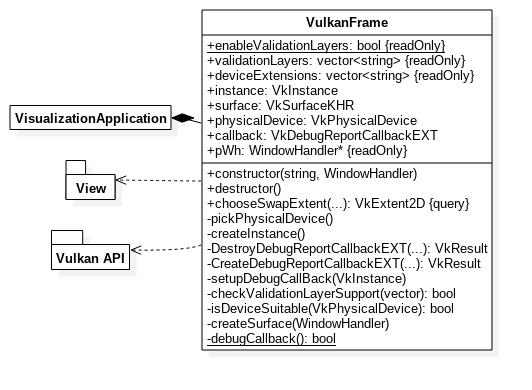
\includegraphics[width=\textwidth]{Model__VulkanFrame_2}
	\centering
	\caption{A \code{VulkanFrame} oszt\'alydiagramja}
\end{figure}
Ez az oszt\'aly felel\H ose, hogy a sz\'amol\'o \'es a rajzol\'o r\'esz k\"oz\"osen haszn\'alt eszk\"ozeit \"osszefogja. Hozza l\'etre a Vulkan Instance-t, illetve v\'alasztja ki az alkalmaz\'as ig\'enyeinek megfelel\H o fizikai eszk\"ozt. Illetve ez szerzi meg az ablakkezel\H ot\H ol a rajzol\'asi fel\"uletet is, amit majd a rajzol\'o oszt\'aly a prezent\'al\'ashoz haszn\'al.

\paragraph{A utility n\'evt\'er}
\begin{figure}[h]
	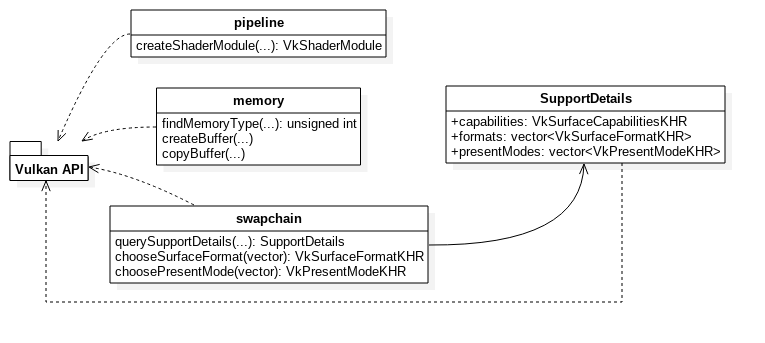
\includegraphics[width=\textwidth]{Model__Utility__Utility_6}
	\centering
	\caption{A \code{utility} n\'evt\'er tartalma}
\end{figure}
Ebben a csomagban seg\'edf\"uggv\'enyek tal\'alhat\'oak a Vulkan-t haszn\'al\'o oszt\'alyokhoz. Azok a met\'odusok ker\"ultek ide, amelyek a sz\'am\'it\'asi \'es a grafikai r\'eszben is m\H uk\"od\'es\"ukben hasonl\'oak, \'igy megfelel\H o param\'eterez\'essel \'altal\'anos\'itani lehetett \H oket vagy csak logikailag valamilyen szinten elk\"ul\"on\'ithet\H oek voltak a f\H o oszt\'alyt\'ol.

H\'arom tov\'abbi r\'eszre bonthat\'o.
\subparagraph{pipeline}
A szerel\H oszalagok l\'etrehoz\'as\'aval kapcsolatos seg\'edf\"uggv\'enyek.

\subparagraph{memory}
Vulkan mem\'oriakezel\'es\'e\'ert felel\H os met\'odusok.

\subparagraph{swapchain}
A swapchain l\'etrehoz\'as\'at seg\'iteni hivatott elj\'ar\'asok \'es f\"uggv\'enyek.

\subsubsection{Fejleszt\'esi lehet\H os\'egek}
A forr\'asf\'ajlokban \code{//TODO:...} kommentekkel jeleztem a k\"ul\"onb\"oz\H o j\"ov\H obeli fejleszt\'esi lehet\H os\'egeket. Ezek k\"oz\"ott vannak kisebb \'es nagyobb m\'ert\'ek\H uek. 
Itt kiemelek n\'eh\'anyat a teljess\'eg ig\'enye n\'elk\"ul:
\begin{itemize}
	\item Az \code{AudioHandler} oszt\'aly absztrah\'al\'asa, \'igy p\'eld\'aul k\"ul\"onbontani a tesztel\'es, \'es a val\'odi mikrofonbemenet r\'eszt. \newline
	M\'asik lehet\H os\'eg, hogy a tesztel\'es r\'esz\'et teljesen kivenni, \'es tesztelni a rendszer be\'all\'it\'as\'aval, hogy az audio outputot audio inputk\'ent is kezelje, ez\'altal biztos\'itani, hogy a program determinisztikuss\'ag\'at.
	\item NVIDIA fejleszt\H ok \href{https://developer.nvidia.com/vulkan-memory-management}{javaslata} alapj\'an a k\"ul\"onb\"oz\H o Vulkan komponensek haszn\'aljanak k\"oz\"os mem\'ori\'at illetve buffereket, eltol\'asokat haszn\'alva, a hat\'ekonys\'ag jav\'it\'asa \'erdek\'eben.
	\item Triple buffering implement\'al\'asa double buffering helyett, \'es megvizsg\'alni, hogy ez mik\'ent v\'altoztat a teljes\'itm\'enyen.
\end{itemize}
